\begin{frame}{Activité: Le crêpier psycho-rigide}

  \begin{block}{Matériel}
    \begin{itemize}
    \item des planchettes en bois de tailles et de couleurs différentes (faces reconnaissables)
    \item éventuellement une pelle à tarte pour retourner les planchettes
    \end{itemize}
  \end{block}

  \begin{block}{Règle du jeu}
    \begin{itemize}
      \item \structure{Installation :} Faire une pile désordonnée de crêpes.
      \item \structure{Objectif :} ranger les crêpes de la plus grande (en dessous) à la plus petite (au dessus), face colorée vers le haut.
      \item \structure{Coup autorisé :} prendre une ou plusieurs crêpes sur le haut de la pile, et de les reposer à l'envers.
    \end{itemize}
  \end{block}

  \bigskip \bigskip \bigskip

  \begin{center}
    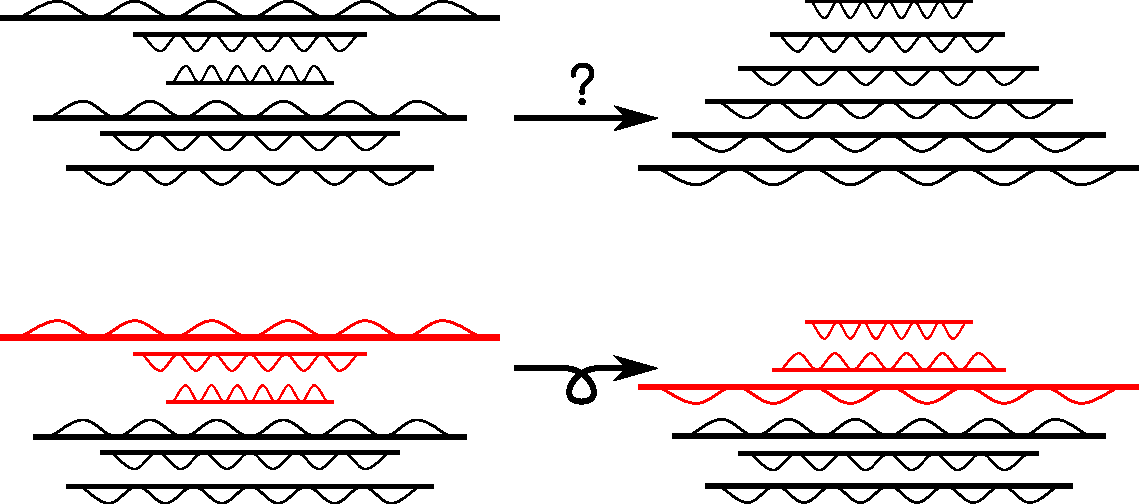
\includegraphics[width=0.8\linewidth]{img/crepier.pdf}
  \end{center}

\end{frame}

\begin{frame}{Ce qu'il faut retenir du  crêpier psycho-rigide}

  \begin{block}{Un algorithme}
    \begin{itemize}
    \item n'a d'intérêt que si on peut l'expliquer
    \item doit être suffisamment simple pour pouvoir l'expliquer à une machine
    \item \alert{\textbf{«Diviser pour mieux régner»}} : on essaie toujours de décomposer un algorithme en tâches simples
    \end{itemize}
  \end{block}

  \begin{block}{L'algorithme que doit suivre le crêpier est :}
    \begin{itemize}
    \item ramener la plus grande crêpe en haut de la pile
    \item retourner pour que la face brûlée soit vers le haut
    \item retourner la pile de sorte à mettre la plus grande crêpe en bas
    \item réitérer avec la crêpe de taille inférieure
    \end{itemize}
  \end{block}

  \begin{block}{Le rapport avec l'informatique}
    \begin{itemize}
    \item l'informaticien passe son temps à trouver des algorithmes et  à les expliquer à la machine
    \item le principe \alert{\textbf{«Diviser pour mieux régner»}} est fondamental en informatique
    \end{itemize}
  \end{block}
\end{frame}

%%% Local Variables: 
%%% mode: latex
%%% TeX-master: "CSIRL"
%%% End: 
